\documentclass[a4paper,12pt,oneside]{book}

%-------------------------------Start of the Preable------------------------------------------------
\usepackage[english]{babel}
\usepackage{blindtext}

%package for hyperlinks
\usepackage{hyperref}
\hypersetup{
    colorlinks=true,
    linkcolor=blue,
    filecolor=magenta,      
    urlcolor=cyan,
}

\urlstyle{same}
%use of package fancy header
\usepackage{fancyhdr}
\setlength\headheight{26pt}
\fancyhf{}
\lhead{\rightmark}
\rhead{
\includegraphics[width=1cm]{images/logo}}
\fancyfoot[RE, RO]{\thepage}
\fancyfoot[CE, CO]{\href{http://www.e-yantra.org}{www.e-yantra.org}}

\pagestyle{fancy}

%use of package for section title formatting
\usepackage{titlesec}
\titleformat{\chapter}
  {\Large\bfseries} % format
  {}                % label
  {0pt}             % sep
  {\huge}           % before-code
 
%use of package tcolorbox for colorful textbox
\usepackage[most]{tcolorbox}
\tcbset{colback=cyan!5!white,colframe=cyan!75!black,halign title = flush center}

\newtcolorbox{mybox}[1]{colback=cyan!5!white,
colframe=cyan!75!black,fonttitle=\bfseries,
title=\textbf{\Large{#1}}}

%use of package marginnote for notes in margin
\usepackage{marginnote}
\usepackage{float}

%use of packgage watermark for pages
\usepackage[scale=2,opacity=0.1,angle=0]{background}
\backgroundsetup{
contents={
\includegraphics{images/logo.png}}
}

%use of newcommand for keywords color
\usepackage{xcolor}
\newcommand{\keyword}[1]{\textcolor{red}{\textbf{#1}}}

%package for inserting pictures
\usepackage{graphicx}

%package for inserting code snippets
\usepackage{listings}

%package for highlighting
\usepackage{color,soul}

% No hyphens while justyfying
\usepackage[none]{hyphenat}

% package for inserting table
\usepackage{tabularray}
\usepackage{ragged2e}

%new command for table
\newcommand{\head}[1]{\textnormal{\textbf{#1}}}


%----------------------End of the Preamble---------------------------------------

\begin{document}

%---------------------Title Page------------------------------------------------
\begin{titlepage}
\raggedright
{\Large e-YSIP 2022\\[1cm]}
{\Huge\scshape FPGA for Edge \\[.1in]}
\vfill
\begin{flushright}
{\large Anupam Kurien Mathew \\}
{\large Dan Mani Binu \\}
{\large Hari Vikinesh \\}
{\large \vspace{0.5cm} \textbf{Mentors \\}}
{\large Isha Kamone \\}
{\large Lohit Penubaku\\}
{\large Duration of Internship: $ 06/06/2022 - 23/07/2022 $ \\}
\end{flushright}

{\itshape 2022, e-Yantra Publication}
\end{titlepage}
%-------------------------------------------------------------------------------

\chapter[FPGA for Edge]{FPGA for Edge}
% New Section
\section*{Abstract}
FPGAs are steadily entering into the race of compute-intensive work precisely in the field of Machine Learning which is referred to as hardware accelerators. These accelerators can improve the performance of the ML Model significantly compared with traditional computing devices like CPU and GPU. FPGAs are preferred because of the hardware reconfigurability, power efficiency and low cost compared to CPUs and GPUs. This project aims to understand and exploit the potential of FPGAs in the application of agriculture. The project focused on training ML models which can be deployed on FPGA, and video processing to use the ML models for indoor agricultural applications. At First, the performance of various ML Models is studied for agricultural applications. In this project ML model is studied and developed for tomato leaf detection. Though there are multiple ML Models available on the air to use, none of them can be used directly on the FPGAs. The ML Model to be chosen should meet the resource constraints of the FPGAs that are bound to be used. Also, FPGAs require sophisticated architecture to run any ML Model. The development of application-specific architecture improves the performance of the model significantly. So, it is important to choose an appropriate ML model to use on FPGA. By analyzing various algorithms considering the constraints. In this project, a YOLOv2-Tiny model is developed from scratch to detect tomato leaves using FPGA and their performance parameters are being measured. A comparison study between FPGA, CPU \& GPUs is also added to this project. This comparison study shows the performance improvement that the FPGA can afford.
\subsection*{Completion status}
Though, this project aimed to do video processing on FPGA. Unfortunately, this project ended up deploying ML models on images and comparing the results of it with CPUs and GPUs.

% New Section
\section{Hardware parts}
This section discusses the hardware parts that are being used in this project along with their descriptions and key features. In this project, two FPGA SoC boards are utilized to measure the performance of the ML Model.
\subsection*{ZedBoard}
ZedBoard is one of the famous FPGA SoC released on 2011 by Avnet. It has an ARM processing system along with Zynq-7000. FPGA Part – XC7Z020-clg-484-1. Features of ZedBoard are as follows.
\begin{itemize}
    \item 512MB DDR3
    \item 256Mb Quad-SPI Flash
    \item Onboard USB-JTAG Programming
    \item 10/100/1000 Ethernet
    \item USB OTG 2.0 and USB UART
    \item PS \& PL I/O Expansion(FMC, 5*Pmod, XADC)
    \item Displays(1080p HDMI, 8-bit VGA, 128x32 OLED)
    \item I2S Audio CODEC
\end{itemize}
A detailed description of this board is given in the reference \href[page=1]{./datasheet/Zedboard_Manual.pdf}{manual} and this board can be purchased using this vendor \href{https://www.avnet.com/wps/portal/us/products/avnet-boards/avnet-board-families/zedboard/}{link}. Figure \ref{figure:zed} shows zedboard.
\begin{figure}[h!]
    \centering
    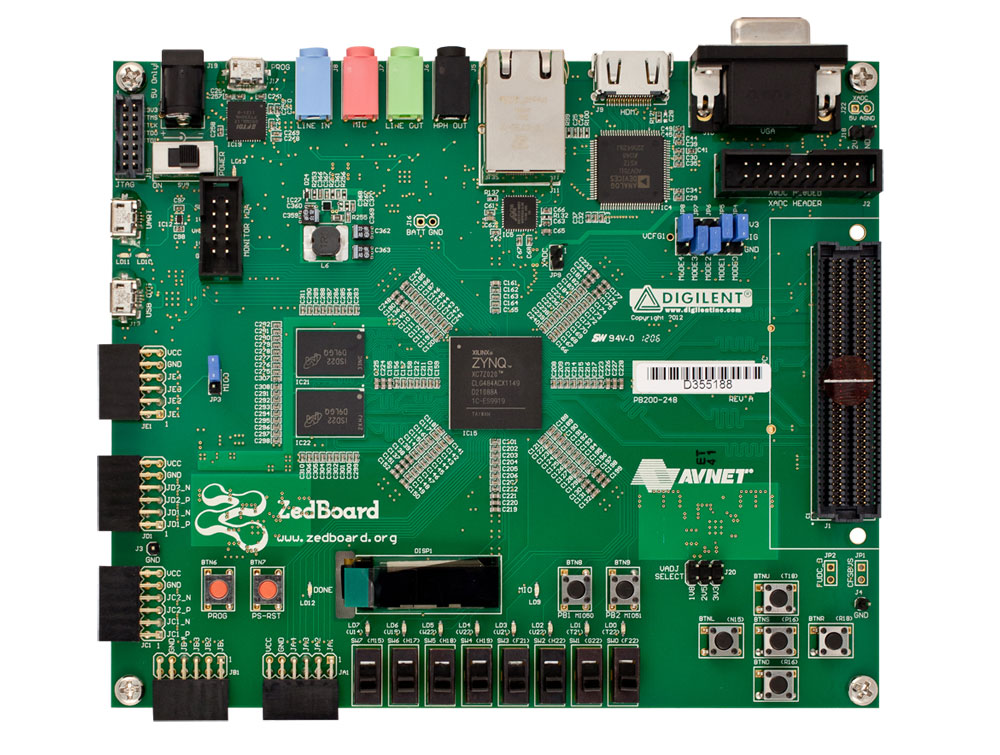
\includegraphics[scale=0.205]{images/zedboard.jpg}
    \caption{ZedBoard}
    \label{figure:zed}
\end{figure}

\subsection*{Nexys Video board}
Nexys Video is based on Artix-7 FPGA released on 2015 by Digilent. A softcore Microblaze processor is prsent as processing system integrator. FPGA Part – XC7A200T-1SBG484C. Features of Nexys Video Board are as follows.
\begin{itemize}
    \item 512MB DDR3
    \item 32Mb Quad-SPI Flash
    \item USB Host, USB UART and USB programming
    \item 10/100/1000 Ethernet
    \item 3.75Gbps GTP transceivers
    \item FMC, 4*PMOD \& XADC
    \item Displays(1080p HDMI In, HDMI Out, 128x32 OLED)
    \item I2S Audio CODEC
\end{itemize}
A detailed description of this board is given in the reference \href[page=1]{./datasheet/Nexys-Video_Manual.pdf}{manual} and this board can be purchased using this vendor \href{https://digilent.com/reference/programmable-logic/nexys-video/start}{link}. Figure \ref{figure:nexysvideo} shows Nexys Video Board.
\begin{figure}[h!]
    \centering
    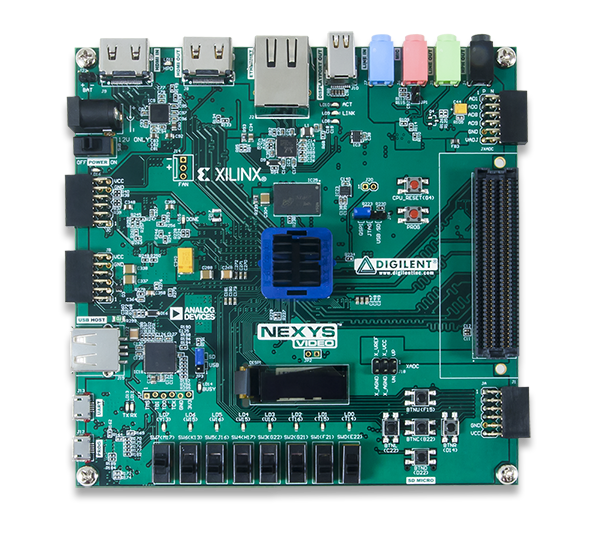
\includegraphics[scale=1.75]{images/nexys-video.png}
    \caption{Nexys Video Board}
    \label{figure:nexysvideo}
\end{figure}

% New Section
\section{Software Setup}
\label{setup}
This section describes all the software that is required to run the project on the FPGA and measure the output performance of the CPU \& GPUs.
\begin{itemize}
    \item \textbf{Vivado HLS} – This software is used to write C/C++ codes in it and then it can synthesize the code to RTL design. It is also possible to simulate the C Code using a C simulator as well as RTL Simulator. After simulation and synthesis, this software can convert the code into an IP block.
    \item \textbf{Vivado} – This software acts as a top entity and this software acts as an architect to design the top-level module design and generate bitstream to implement them on hardware. In this software, the generated IP blocks can be used to create a design or users can use HDL languages like Verilog or VHDL to generate a bitstream file. One main advantage of this software is it supports mixed language implementations which means users can use both Verilog and VHDL in the same design. The top-level design can be exported as hardware design as well.
    \item \textbf{Xilinx SDK} – This software is used to run the hardware design as a bare-metal application on the FPGAs. This software is used if the user has processing system parts involved in the design. The user should create a separate project to program this processing system part.
    \item \textbf{Paperspace} – Paperspace is a cloud computing service developed for Machine Learning and other compute-intense tasks to run on the cloud GPUs. This organization provides Cloud GPUs at a low cost. They provide CPUs and GPUs for usage at cost on an hourly/monthly basis. The GPUs are ranges from Nvidia M4000 to A100 models. In this project, an Nvidia A4000 model is provided for the development and testing of the ML Model.
\end{itemize}
Apart from the software mentioned above. There are certain python modules needed to be installed to run the model which are mentioned below.
\begin{itemize}
    \item mathplotlib - interactive graph creater module
    \item Tensorflow - ML Traing and Testing module
    \item pyserial - Serial Read module
\end{itemize}
Also, powerstat linux tools are required to measure the power consumption.

\subsection*{Installation Steps}
\begin{enumerate}
    \item Visit this \href{ https://www.xilinx.com/support/download/index.html/content/xilinx/en/downloadNav/vivado-design-tools/archive.html}{link}. Scroll down and click on 2018.3 Archive.
    \item Choose the third option to download the software. Refer Figure \ref{figure:HLx}.
        \begin{figure}[h!]
            \centering
            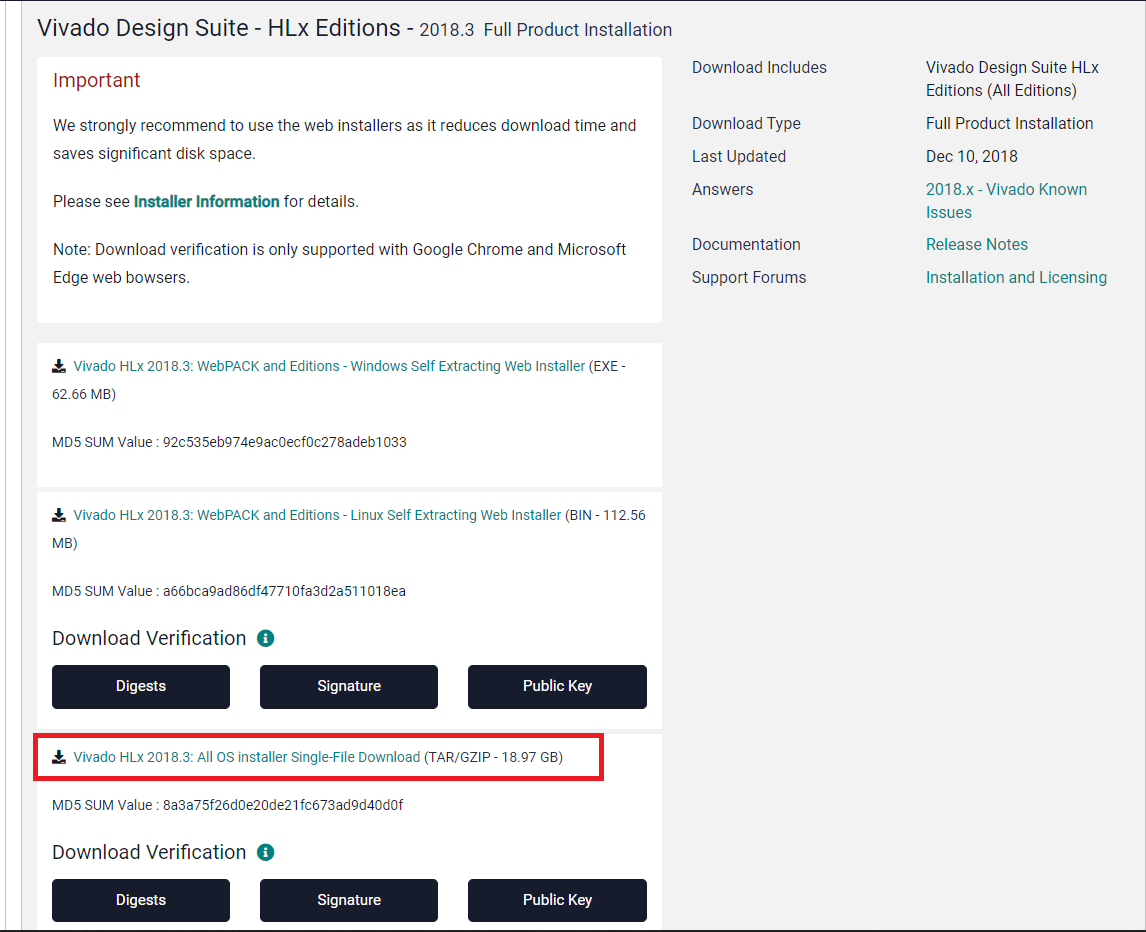
\includegraphics[scale=0.5]{images/HLx_download.png}
            \caption{Xilinx Vivado Download Page}
            \label{figure:HLx}
        \end{figure}
    \item If a login prompt appears log in using the Xilinx account and the download will start automatically.
    \item After downloading the software, Extract it. Now, the xsetup.exe file should be present inside the folder.
    \item After the installer appears. On the First Page, Click on Next. On the license agreement tab, accept all license agreements and click on Next.
    \item Now, Choose Vivado HL Design Edition and click on Next.
    \item Click on Next and in the next tab choose the appropriate location (prefer SSD) to install the software.
    \item Finally, on the next tab click on the Install button to install the software.
\end{enumerate}

% New Section
\section{Model Development}
This section of the report explains the development of the custom model for tomato leaf detection using object detection algorithms. The details for building a Hardware accelerator are also described in detail.

\subsection*{Object Detection}
Object detection is a computer vision technique for locating instances of objects in images or videos. All the Object detection algorithm uses Machine Learning Techniques to detect some objects and produce meaningful results. Some popular object detection algorithms are R-CNN, SSD, and YOLO algorithms. To detect an object using these algorithms requires a pre-trained network. This pre-trained network is called a base model or weights of the network. In this project, to detect tomato leaves YOLOv2-Tiny model has been used. At the start of the project, different tomato leaf detection models are developed such as YOLO-v5, YOLO-v3 tiny and mask-r-CNN. The results of these models are shown in the figure \ref{figure:detectionresults}. At Later stage of the project models for yolo-v2 and SSD mobilenet are also developed. In comparing the results from various models with the model size, the YOLOv2-Tiny model is chosen. The model size is a critical parameter because FPGAs have limited resources.
\begin{figure}[h!]
    \centering
    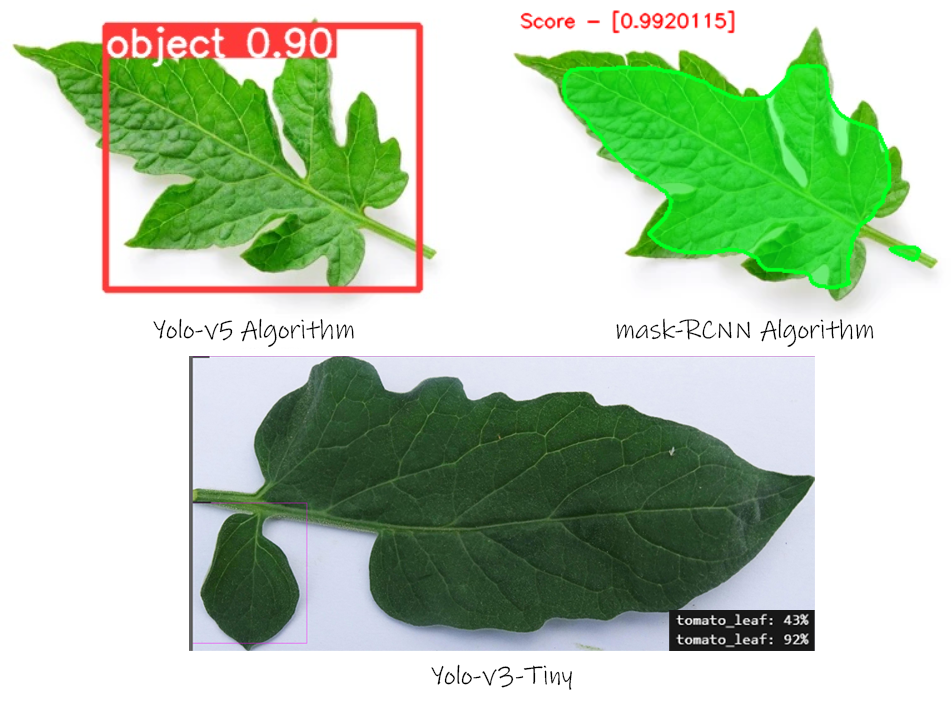
\includegraphics[scale=0.325]{images/models.png}
    \caption{Initial Model Results}
    \label{figure:detectionresults}
\end{figure}

\subsection*{YOLOv2-Tiny Architecture}
YOLOv2-Tiny gives state-of-the-art detection accuracy on the PASCAL VOC and COCO. It can run on varying sizes offering a tradeoff between speed and accuracy. The dataset used for this project is the village plant dataset and modified to PASCAL VOC format only for healthy tomato leaves. This model is trained in the Paperspace platform. The figure \ref{figure:yolov2} shows the architecture of YOLOv2 that is used in this project.
\begin{figure}[h!]
    \centering
    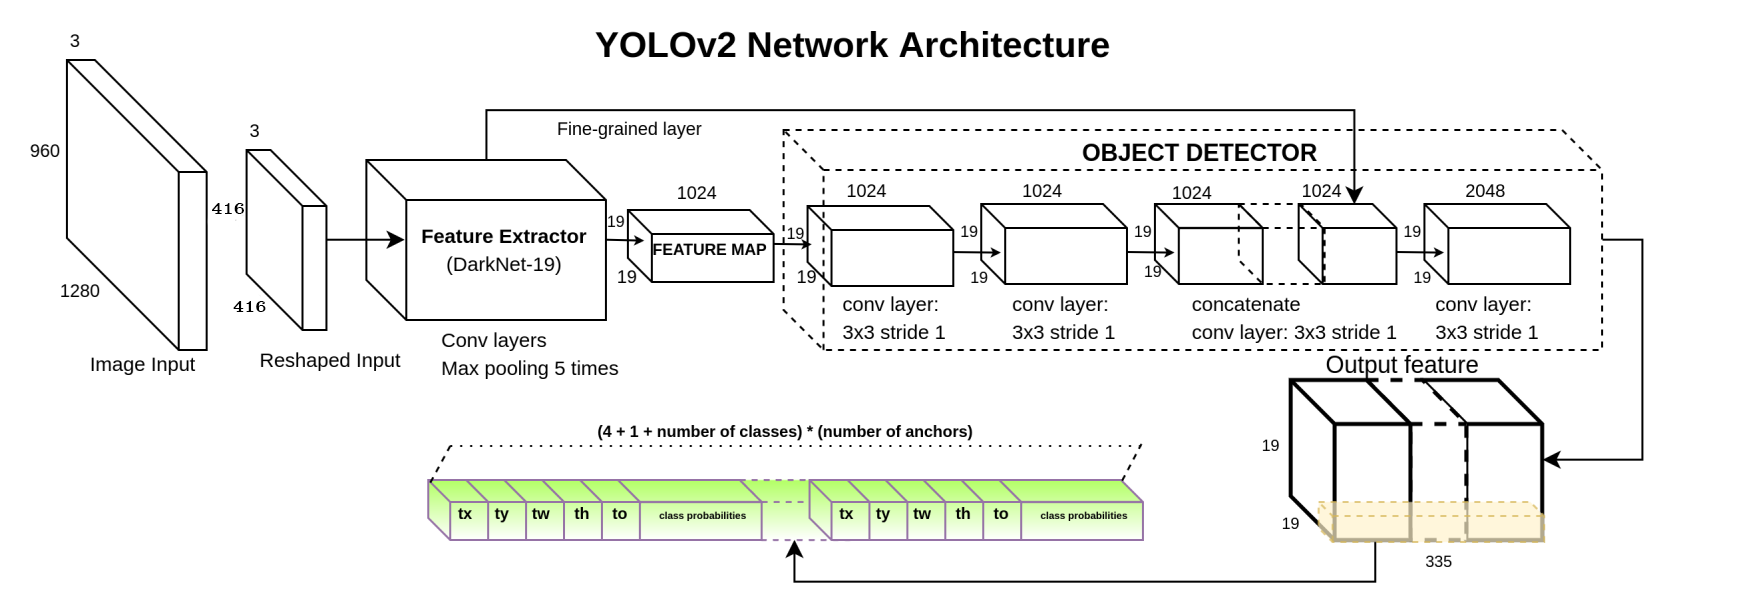
\includegraphics[scale=0.21]{images/yolov2-architecture.png}
    \caption{YOLO-v2 Architecture}
    \label{figure:yolov2}
\end{figure}

\subsection*{Hardware Accelerator}
An Object detection model cannot be implemented on the FPGAs directly. So, a Hardware Accelerator must be developed to run the model. So, a custom hardware accelerator for FPGA is developed to detect tomato leaves using the YOLOv2-Tiny model. This Accelerator uses Vivado HLS pipelining tools to reduce the overall execution time significantly and manages memory utilization. The basic architecture of our model is shown in the figure \ref{figure:architecturetop}. The output result of this accelerator is sent to the laptop for visualization using UART Communication.
\begin{figure}[h!]
    \centering
    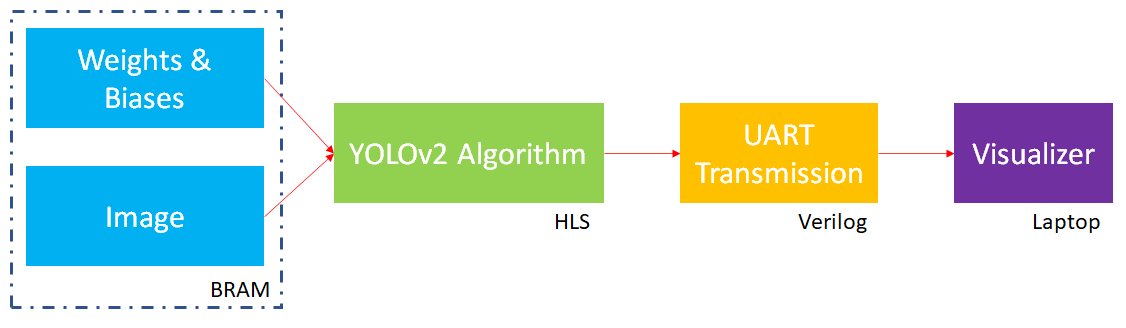
\includegraphics[scale=0.3]{images/architecturetop.png}
    \caption{Hardware Accelerator}
    \label{figure:architecturetop}
\end{figure}

% New Section
\section{Code Explanation}
All the codes that are used in this project are described in this section. The code explanation part is split into four parts namely python notebooks, python scripts, HLS Codes and Verilog HDL. Python scripts are used to test the model and obtain the results of the YOLO-v2 model. HLS Codes are used to develop the hardware accelerators for FPGA deployment. Verilog HDL is used to transmit the output of the hardware accelerator to the laptop. Necessary files and codes to replicate this project is added to the GitHub repository and it can be accessed using this \href{https://github.com/hari-vickey/FPGA-for-Edge}{link}.

\subsection*{Python Notebooks}
\textbf{Notebook 1} - yolov2-tiny.ipynb\vspace{0.2cm}\\
This Notebook is used to train the yolov2 algorithm using the darknet. This notebook has the necessary comments to develop a custom model and convert it to the Keras model at the end. This notebook uses the pre-trained network to train a new model. Important code snippets for training and testing is mentioned below.\vspace{0.2cm}
\begin{lstlisting}
# Start Training
# users are free to use custom configurations or use
# prebuilt configuration files under /darknet/cfg 
# directory

!./darknet detector train yolov2.data \
    cfg/<custom_cfg>.cfg \
    yolov2.weights -dont_show

# Test the trained model using a darknet detector 
# and use appropriate paths
!./darknet detector test yolov2_tiny.data \
    cfg/yolov2_tiny.cfg \
    backup/yolov2_tiny_last.weights \
    test/11.jpg

# Convert weights to a Frozen Graph
# Darkflow repository is used
!./flow --model /<path>/yolov2_tiny.cfg \
    --load /<path>/yolov2_tiny.weights --savepb

\end{lstlisting}
\textbf{Notebook 2} - yolov2-scratch.ipynb\vspace{0.2cm}\\
This notebook is used to develop and test the yolov2 algorithm from scratch as it is using very minimum external modules. Also, the functions for the algorithm are written in such a way that they can be converted to C/C++ code for HLS implementation. This notebook has all the functions to load the yolov2 model and detect bounding boxes using the yolov2 regressor.\vspace{0.2cm}
\begin{lstlisting}
# Recreate the exact same model, including its weights
and the optimizer
new_model = tf.keras.models.load_model('yolov2-tiny.h5')

# Show the model architecture
new_model.summary()

def padding(X, pad,n_H,n_W,n_C): 
    the function creates a layer of zeroes around
    the entire 2D matrix. The following function
    is modified for padding in 1 dimension.
    X   - array to be padded with zeros
    pad - the width of padding
    n_H - height of the 1D array in 2D form
    n_W - width of the 1D array in 2D form
    n_C - no of channels in image
    X_pad - output array which whose dimensions
    have been increased to (n_H/n_C + 2*pad)

def convolution(k_width ,k_height ,filters, arr_width,
        arr_height  ,arr_channels ,arr ,s , k):
  performs normal convolution on the array/image passed
  the function performs a horizontal convolution first
  throught the entire image and then performs vertical
  convolution
  k_width      - kernel width
  k_heigth     - kernel height
  filters      - the no of kernel filters applied
  to the image/array
  arr_width    - width of the array
  arr_height   - height of the array
  arr_channels - no.of channels in the passed array
  arr          - the image/array on which convolution
  is to be performed
  s            - stride
  k            - the kernel weights as 1D array
  arra         - final output after convolution

def batch_norm(X,arr_channels,arr_height,arr_width,K):
   batch normalization performs - 
        1. subtraction with moving mean indicated by
                 K[2*arr_channels+j]
        2. division with root of standard deviation 
        indicated by math.sqrt(K[3*arr_channels+j])
        3. multiplication by Gamma indicated by K[j]
        4. addition by Beta indecated by 
                K[1*arr_channels+j]

    X            - array to be batch normalized
    arr_channels - no.of channels in array
    arr_height   - height of the array in 2D
    arr_width    - height of the array in 2D
    K            - Batch normalization weights in the
                   order gamma, beta, standard deviation,
                   subtraction
    X            - calculations performed in the same array
                   and returned as output

def max_pooling(k_width = 2, k_height = 2, filters = 3,
        arr_width = 8, arr_height =8 ,arr_channels = 3,
        arr = img,s = 2):
    Max Pooling calculates the maximum value for patches 
    of a feature map, and uses it to create a downsampled
    feature map. In and Outs are similar to convolution.

def leaky_relu(alp, arr):
  leaky relu returns same number if the number is greater
  than 0 else returns the number after multiplying it alp.
  alp - computation parameter
  arr - the array on which leaky relu is to be performed
  arr - also returned as output

\end{lstlisting}

\subsection*{Python Scripts}
\textbf{Python Script 1} - visualize.py\vspace{0.2cm}\\
This code is used to get the results from the Hardware accelerator of the FPGA using the serial communication protocol(UART). This code reads the data from the serial port and decodes it to show the detection result using OpenCV. Main parts of the code are attached below.\vspace{0.2cm}
\begin{lstlisting}
# Open Serial Port
ser = serial.Serial('COM6', 115200, timeout=1)
# Reading Serial data
while True:
    # Reading a Line Input
    message = ser.readline()
    if message:
        # Converting Byte String to unicode string 
        data = message.decode()
        break

# Draw Bounding Box and label it
img = cv2.rectangle(img, (int(data[3]), int(data[4])),
    (int(data[5]), int(data[6])), (255,0,0), 1)
img = cv2.putText(img, data[2], (int(data[3]),
    int(data[4])+25), cv2.FONT_HERSHEY_SIMPLEX,
    0.9, (0,0,255), 1)
\end{lstlisting}
\textbf{Python Script 2} - convertImage.py\vspace{0.2cm}\\
This code is used to convert the input RGB image into a single dimension array. This array is stored in the C header file using this script.\vspace{0.2cm}
\begin{lstlisting}
# Function File Header Writer
def file_write(file, data, h, w, c):
    This function will write a header file to store images.
    file - path with filename
    data - image data
    norm - Normalization
    h    - height
    w    - width

# Converting 3d Array to 1d list
for i in range(0, h):
    img_linear = []
    for j in range(0, w):
        for k in range(0, c):
            img_linear.append(img[i][j][k])
    row_array.append(img_linear)
\end{lstlisting}
\textbf{Python Script 3} - yolov2-tiny.py\vspace{0.2cm}\\
This code is used to run the yolov2-tiny algorithm on the CPU and GPU to analyze the performance of the model. The yolov2-tiny model is converted to TensorFlow frozen graphs for implementation. The output of this code returns the leaf detection bounding boxes along with the accuracy and latency.\vspace{0.2cm}
\begin{lstlisting}
def main():
    This function loads the yolov2-tiny model using the 
    tensorflow. After that, this function will call
    other funtions to detect the tomatoleaf in given
    image. The Output image is displayed using the 
    matplotlib library. This function also calculates 
    the latency of the model.

def get_input_data(img_file):
    This function will read the input image using the
    PIL library and convert the image to a normalized
    float32 numpy array.
    input:
        img_file - path to input image
    returns:
        new_image  - resized image
        input_data - normalized numpy array

def check_result(data):
    This function interprets the numpy array and apply 
    bounding box regressor of the yolo architecture to
    finalize outputs. This function instatiates small
    math functions to calculate results.
    input:
        data - normalized numpy array
    returns:
        output - predictions
\end{lstlisting}
\subsection*{HLS Codes}
\textbf{HLS Code 1} - yolov2.cpp\vspace{0.2cm}\\
This code is the brain of the custom hardware accelerator and this code detects the tomato leaf based on the trained model and input image using the yolov2 architecture. The regressor for yolov2 algorithm is described below.\vspace{0.2cm}
\begin{lstlisting}
// Defining Custom Datatype
typedef ap_int<9> bbxy;
typedef ap_int<10> accuracy;
typedef ap_int<1> int1;
typedef ap_int<3> int3;

// Declaring Output Products
bbxy bbx1, bby1, bbx2, bby2;
accuracy score = 0;
int3 leaves = 0, flag = 0;
int1 result = 0;

void yolo_eval(float *box_xy, float *box_wh, 
    float *box_confidence, float  *box_class_probs,
    float *boxes,float *box_class_scores,
    float threshold, int &count)

    Function Name: yolo_eval
    Input        : 
   -- Yolo Outputs --
   box_xy        - bounding box x and y position
   box_wh        - bounding box widht and height values
   box_confidence- confidence of the bounding boxes
   box_class_prob- detected class probability
   --               --
   boxes            - maximum predicted box_whes
   box_class_scores - bounding box class scores
   threshold        - threshold for scores
   count            - counter
   Description  : This function converts yolo outputs 
   (multiple bounding boxes) to best predicted bounding
   box along with their scores, box co-ordinates and
   classes.

void non_max_suppresion(float *scores,float *boxes,
        int count, int max_boxes = 10,
        float iou_threshold = 0.3)
    Function Name: non_max_suppresion
    Input        : 
    scores        - scores array
    boxes         - bounding boxes array
    count         - count value
    max_boxes     - maximum no of bounding boxes
    iou_threshold - threshold for intersection over union

    Description  : This function validates all the input 
    bounding boxes and outputs the more appropriate 
    bounding box for the input parameters.

int yolov2Algorithm()
    Function Name: yolov2algorithm
    return       : output flag
    Description  : Function to perform yolo operations
                   it calls appropriate functions to do
                   convolution for the given input images.
int regressor()
    Function Name: regressor
    return       : output flag
    Description  : This function stores parameters for
    yolov2 regressor and calls appropriate functions
    to complete evaluation and give the final results.

void hlsTop(int1 start, int1 &compute, int3 &leaves,
        accuracy &scores_out, bbxy &out_bbx1, bbxy &out_bby1,
        bbxy &out_bbx2, bbxy &out_bby2)
    Function Name: hlsTop
    Input        : start - start switch
    Output       :
    compute - start tx computation flag
    leaves  - no of leaves detected flag
    scores_out - accuracy of detected leaves
    out_bb--   - bounding box co-ordinates
    Description : This function will create the module I/Os
    using the HLS Pragmas.
\end{lstlisting}
\subsection*{Verilog HDL}
\textbf{Verilog Code 1} - uart\_tx.v\vspace{0.2cm}\\
This module is responsible to get input from the ssd model and
convert the decimal value to digits for UART transmission. Then,
this module transmits the necessary signals for the uart\_tx module
to send the data serially.\vspace{0.2cm}
\begin{lstlisting}
Inputs
clock      - 100Mhz Clock
reset      - restart computation
result     - model identification flag
compute    - start flag for computation
imgID      - image Number
accuarcy   - Model's score
bbxn, bbyn - co-ordinates of the boundary boxes
Outputs
tx         - serial data output pin
txComplete - transmission status
\end{lstlisting}
\textbf{Verilog Code 2} - uart.v\vspace{0.2cm}\\
This module is responsible for transmitting the message through
serial communication protocol UART.\vspace{0.2cm}
\begin{lstlisting}
Inputs
clk     - 100MHz on-board Oscillator
reset   - reset to resend serial data
result  - tells the tomato leaf detected or not
imageID - no of the image used
acc_n   - accuarcy in three digit
bb1_n   - boundary box 1 co-ordinates in six digits
bb2_n   - boundary box 2 co-ordinates in six digits
Outputs
txOut  - Serial Output
txDone - Transmission Status
UART Transmission Parameters
baud rate = 115200
clocks per bit (cpb) = (100*10^6)/115200 = 868
start bit = 0, stop bit = 1;
1 start bit, 1 stop bit and no parity bit
// msg Format = #2-1-97.8-213-231-345-322#
- is the delimiter
# is start and stop bit indexes
\end{lstlisting}

% New Section
\section{Demonstration}
This section deals with implementing the hardware accelerator on the FPGA using the step-by-step method. Also, this section lists the steps to obtain the results from the CPU and GPU for comparing the results. A demonstration video is also added to Google \href{https://drive.google.com/file/d/16WsQvynVm7deqsmaAB_vbvT4a0hNm1vk/view?usp=sharing}{Drive} for the users to get a better understanding of the implementation process. All the project files, documents, reference materials and models that are used and carried out throughout the project are added to this Google \href{https://drive.google.com/drive/folders/1BqBZ5q350s5VY3MsdWqtLLzMQtBQPrcu?usp=sharing}{Drive}.

\subsection*{Deploying the Hardware Accelerator}
After generating bitstream using the vivado software, it is ready for deployment. But, before uploading bitstream into the FPGA. The users should run the python program on their laptop or PC. The steps for executing this program are mentioned below with the reference figures.
\begin{enumerate}
    \item Connect the micro-USB data cable to the UART port of Nexys Board and Connect a male to female jumper wire to the JA1 PMOD connector and the RX port of any USB to UART converter.
    % Refer the figure \ref{figure:usb-uart-connection}.
    %     \begin{figure}[h!]
    %         \centering
    %         \includegraphics[width=\linewidth]{}
    %         \caption{USB UART Connection}
    %         \label{figure:usb-uart-connection}
    %     \end{figure}
    \item Open Device Manager on the PC or Laptop and check the COM port. Open the visualize.py program file and make sure that both COM ports are the same.
    % Refer the figure \ref{figure:com-verify}
    %     \begin{figure}[h!]
    %         \centering
    %         \includegraphics[scale=0.5]{}
    %         \caption{COM Port Verification}
    %         \label{figure:com-verify}
    %     \end{figure}
    \item Run the Program in the command prompt or any python IDE.
    % Refer the figure \ref{figure:run-program}
    %     \begin{figure}[h!]
    %         \centering
    %         \includegraphics[scale=0.5]{}
    %         \caption{Run the Program}
    %         \label{figure:run-program}
    %     \end{figure}
    \item Now, Program the FPGA with bitstream using Vivado Software.
    % Refer the figure \ref{figure:program-device}
    %     \begin{figure}[h!]
    %         \centering
    %         \includegraphics[scale=0.5]{}
    %         \caption{Program the Device}
    %         \label{figure:program-device}
    %     \end{figure}
    \item After Accelerator completes the detection, the results are transmitted to the PC and the user should see an output similar to the figure \ref{figure:output-fpga}.
        \begin{figure}[h!]
            \centering
            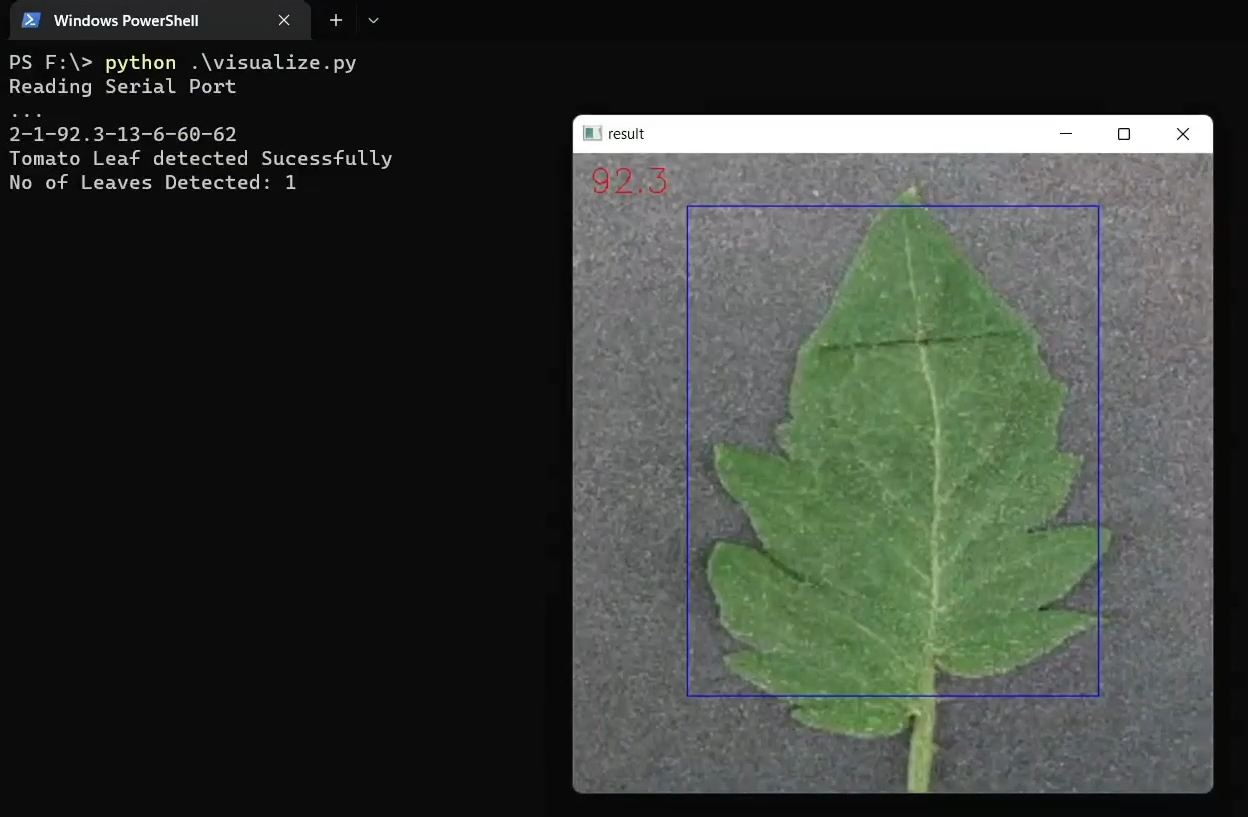
\includegraphics[scale=0.2]{images/output.png}
            \caption{Output of the Accelerator}
            \label{figure:output-fpga}
        \end{figure}
\end{enumerate}

\subsection*{Obtaining Results from the Hardware}
To analyze the results with the Hardware Accelerator, the users can follow the steps mentioned below to obtain the results from the CPU and GPU.\\

To measure the performance of the built YOLOv2 model, the required modules to run and test the program should be installed on the computer. All the required modules are mentioned in \autoref{setup}.\\
To measure the performance of the model follows the steps mentioned below.
\begin{enumerate}
    \item Make sure that tflite model, test images and yolov2-tiny.py are in the same directory.
    \item Open two terminals in separate windows, first run the python program in one terminal and the powerstat tool in another window.
    \item Python program shows the results of the model in the terminal that includes accuracy, class, bounding box and latency.
    \item Parallelly, the power stat tool shows the power consumption of the computer, when the python program is running at the backend the power consumption should be recorded. Refer figure \ref{figure:record-simple}.
    \begin{figure}[h!]
        \centering
        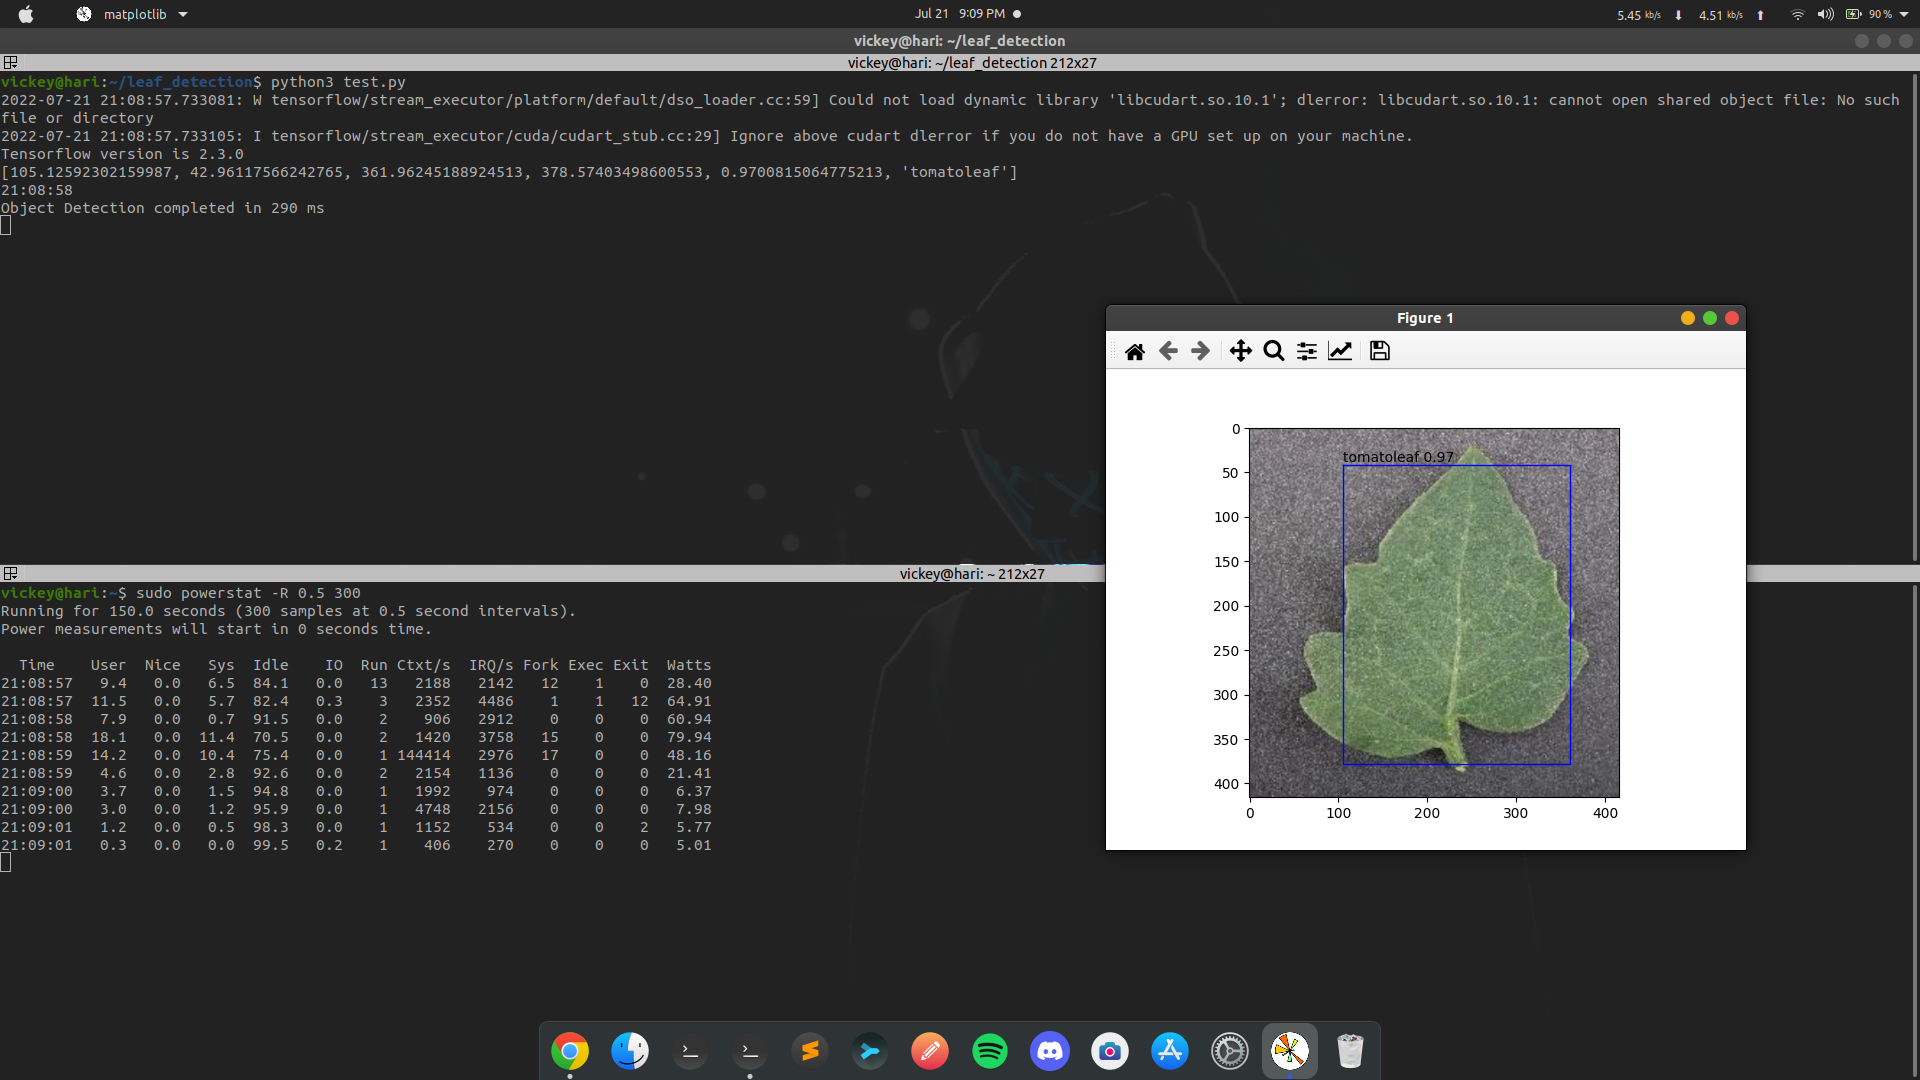
\includegraphics[width=\linewidth]{images/record-perform.png}
        \caption{Sample Recording}
        \label{figure:record-simple}
    \end{figure}
\end{enumerate}

To measure the performance of the model on the FPGA with resource utilization Vivado softwares are used. If the Implementation of the design in the Vivado software completes successfully, then Vivado provides the complete report of the design with the details of resource utilization, peak power consumption and timing constraints. Refer the figure
\begin{figure}[h!]
    \centering
    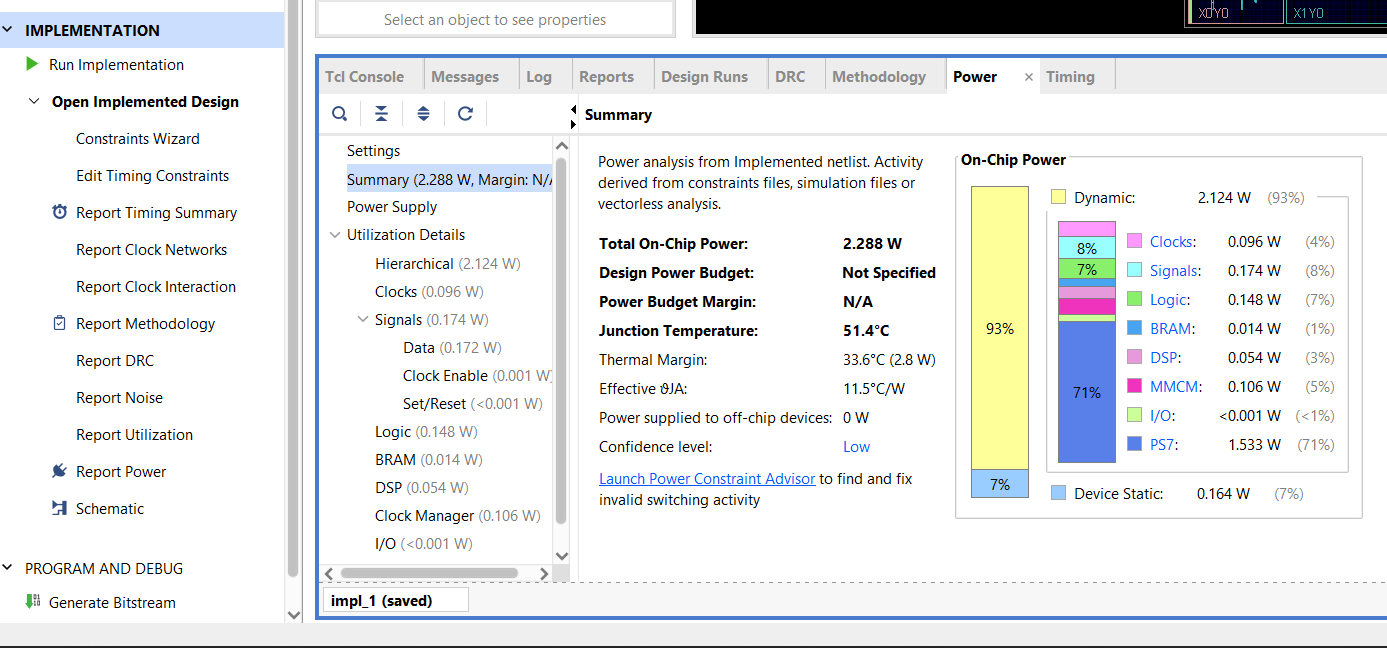
\includegraphics[scale=0.35]{images/record-util.png}
    \caption{Recording Resource Utilization}
    \label{figure:record-util}
\end{figure}

% New Section
\section{Performance Study}
This section studies the results from the implemented Hardware Accelerator and compares the performance with the CPU and GPU. Also, a performance comparison between the implemented design and the existing designs is also analyzed.

\subsection*{Comparison with Traditional Hardwares}
The project laid focus on the comparison between eight hardware, comprising four CPUs
two GPUs and two FPGAs. Latency and Power consumption are the two domains under comparison.

From the Figure \ref{figure:compare-hardware} Among the CPUs, the i7-9750CPU had the least latency of 148ms in implementing YoloV2-tiny while  that of INTEL XENON 2.3GHz was recorded to be the highest (326ms). Both the ZedBoard and Nexys Video latency was recorded to be about 210ms with Nexys Video Board having better performance than Of all devices, GPUs are found to have the least latency, with NVIDIA RTX A4000 running at 124ms latency and NVIDIA Tesla at 84ms.
\begin{figure}[h!]
    \centering
    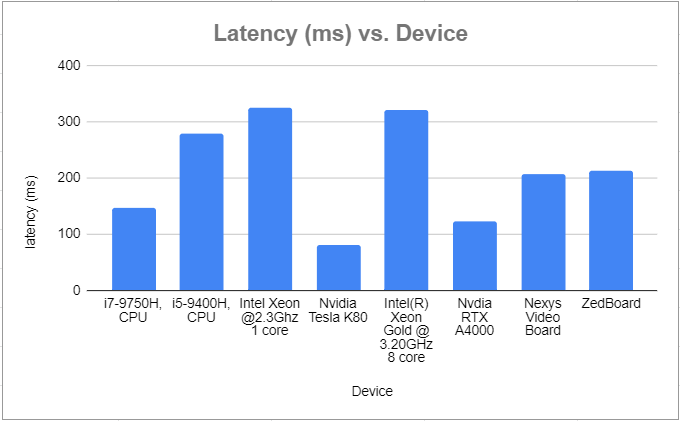
\includegraphics[scale=0.38]{images/hardware-performance.png}
    \caption{Latency Comparison}
    \label{figure:compare-hardware}
\end{figure}

Looking into power consumption from figure \ref{figure:compare-power}, The i7-9750H drinks about 79W of power and the i5-9400H at 59W.
Both the NVIDIA Tesla K80 and NVIDIA RTX A4000 consume a reasonable amount of 43W,
while the Nexys and ZedBoards consume very less power of 3W.

\begin{figure}[h!]
    \centering
    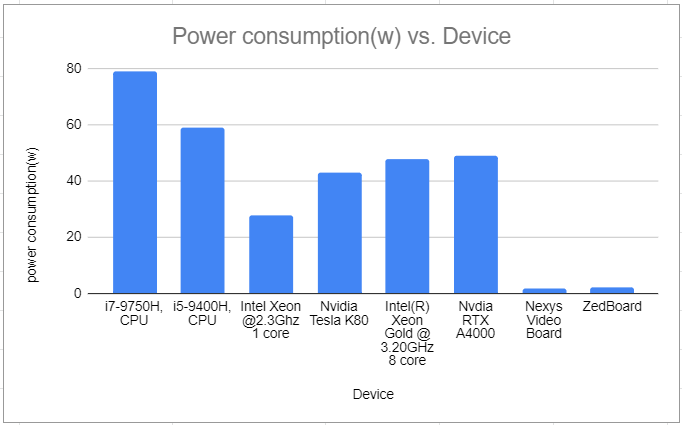
\includegraphics[scale=0.38]{images/power-consumption.png}
    \caption{Power Consumption Comparison}
    \label{figure:compare-power}
\end{figure}

\subsection*{Comparison with Existing Accelerators}
This work used 32-bit floating point representations for weights leading to achieving higher accuracy. This work requires the lowest number of flip flops at 28.5K and 23.8K for ZedBoard and Nexys video board respectively. From the table, BRAM utilization on this work is also lower than that of Kintex Ultrascale (1814 KB) at 846KB for Zedboard and 890KB for Nexys while possessing a bigger image size and cnn size. The DSP utilization for Zedboard is lowest among all hardware accelerators compared at 121 while Nexys board matches that of Zynq ZC702 at 140. The hardware utilization is lower only on accelerators which use a combination of smaller image size and lower precision. In that case, the utilization is lower than Kintex Ultrascale. The other works which use higher image size consequently use significantly higher resources. This translates to those accelerators not being implementable on lower-tier FPGAs.
\begin{table}[H]
    \centering
    \caption{Comparison with Hardware Accelerators}
    \resizebox{\textwidth}{!}{
    \small
    \begin{tblr}{|Q[c,30mm]|Q[c,15mm]|Q[c,15mm]|Q[c,18mm]|Q[c,15mm]|Q[c,15mm]|Q[c,20mm]|Q[c,15mm]|Q[c,15mm]|Q[c,15mm]|}
    \hline
    \textbf{Platform}         & Zynq XC7Z045 & Xilinx Zynq ZC702 & Kintex Ultrascale XCKU115 & Stratix-V   & Virtex-7 VC707     & Zynq Ultrascale+ & Intel Arria 10 GX115 & ZedBoard (This work) & Nexys Video (This work) \\ \hline
    Frequency (MHz)           & 200          & 100               & 125                       & 150         & 200                & 200              & 200                  & 100                  & 100                     \\
    BRAMs (KB)                & 186          & 630               & 1814                      & 2210        & 1214               & 1824             & 2232                 & 846                  & 890                     \\
    DSPs                      & -            & 140               & -                         & 384         & 272                & 2520             & 1518                 & 121                  & 148                     \\
    LUTs                      & 46.3K        & 36.1k             & 392.9K                    & 230.9K      & 104.7K             & 600K             & 138K                 & 51.4K                & 40.2K                   \\
    FFs                       & -            & 36.8K             & 348K                      & 350K        & 140.1K             & -                & 823.4K               & 31.4K                & 31.4K                   \\
    CNN Size                  & 0.1125       & 14.5              & 1.2                       & 1.45        & 30.74              & 5 layers of VGG  & 30.95                & 42.3                 & 42.3                    \\
    Precision                 & 8-bit fixed  & 8-bit fixed       & 8-bit fixed               & 8-bit fixed & (8-16)bit fixed    & 16-bit fixed     & 16-bit fixed         & 32-bit float         & 32-bit float            \\
    Image Size                & 32x32        & -                 & 32x32                     & 224x224     & 224x224            & 224x224          & 224x224              & 64x64                & 64x64                   \\ \hline
    \end{tblr}}
    \label{table:compare-accelerators}
\end{table}

% New Section
\section{Conclusion}
From the comparisons given above, it is evident that ML model implementation works best on FPGAs and GPUs. The choice between FPGA and GPU is application specific. FPGAs are best for low-power implementation and standalone applications. GPUs for low latency models. A more efficient code can alter the speed and resources required to implement the model. Traditional hardware like CPUs has turned out to be poor choices for model implementation. Based on the resource cost and simple architecture the propsed model can be implemented on low-tier FPGAs.

% New Section
\section{Future Work}
This project can act as the baseline for the projects implementing real-time leaf detection using Xilinx FPGAs. This project’s code can be implemented on Zynq and MicroBlaze series FPGAs for performance analysis. It is also possible to develop any custom object detection model and implement it on the other FPGAs using this project.

% New Section
\section{Bug report and Challenges}
In HLS codes there are some parts of the code that are not optimized to the best. Also, the use of variables and their size can be reduced to some extent to reduce bottleneck memory usage on the FPGAs. The UART Verilog code has a decimal to digit converter that has division and modulus operations costing higher resource utilization. So, other methods should be employed to reduce resource utilization.\vspace{0.5cm}\\
An Important challenge our project has is integrating the OV7670 camera into the FPGA. This camera was used at the start of the project. Though the camera interface is proper, the output from the camera is not clear. This is due to improper I2C configuration information provided by the vendor. Some FPGA hobbyists have claimed this issue on the internet. So, this area will be quite tricky for the developers.\vspace{0.5cm}\\
Another challenge is trying to figure out the appropriate model to deploy on the FPGA. This is because of the resource constraints of the FPGAs. Also, memory management is really important to reduce latency for reading and writing operations. If the FPGA tries to access memory from the external DDR or other secondary memory storage devices, it will increase the latency of the entire model.

% References
\begin{thebibliography}{li}
\bibitem{j1}
S Zhang, J Cao and Q Zhang,
{\em An FPGA-Based Reconfigurable CNN Accelerator for YOLO},
2020.

\bibitem{j2}
DT Nguyen, TN Nguyen Hyuk Lee and H Kim,
{\em A High-Throughput and Power-Efficient FPGA Implementation of YOLO CNN for Object Detection},
2019.

\bibitem{j2}
Colleman, Steven, and Marian Verhelst,
{\em High-Utilization, High-Flexibility Depth-First CNN Coprocessor for Image Pixel Processing on FPGA},
2021.

\bibitem{j4}
Sharma, Hardik and Mahajan,
{\em From High-Level Deep Neural Models to FPGAs},
2016.

\bibitem{j5}
K Kara, D Alistarh and G Alonso,
{\em FPGA-accelerated Dense Linear Machine Learning A precision Convergence Trade-off},
2017.

\bibitem{j6}
MA Momen and MAS Khalid,
{\em FPGA-Based Acceleration of Expectation Maximization Algorithm Using High-Level Synthesis},
2019.

\bibitem{j7}
A Sanaullah, C Yang and Y Alexeev,
{\em Real-time data analysis for medical diagnosis using FPGA-accelerated neural networks},
2018.

\bibitem{j8}
S Jiang, D He and C Yang,
{\em Accelerating Mobile Applications at the Network Edge with Software-Programmable FPGAs},
2018.

\bibitem{j9}
S Kala, J Mathew and BR Jose,
{\em UniWiG Unified Winograd-GEMM Architecture for accelerating CNN on FPGAs},
2019.

\bibitem{j10}
X Liu, HA Ounifi and A Gherbi,
{\em A Hybrid GPU-FPGA-based Computing Platform for Machine Learning},
2018.
\end{thebibliography}


\end{document}

